
% Reference: https://tex.stackexchange.com/questions/8827/preparing-cheat-sheets/8915

% Package imports.
\documentclass[10pt,landscape]{article}
\usepackage{multicol}
\usepackage{calc}
\usepackage{ifthen}
\usepackage[landscape, a4paper]{geometry}
\usepackage{amsmath,amsthm,amsfonts,amssymb}
\usepackage{color,graphicx,overpic}
\usepackage{hyperref}
\newenvironment{Figure}
{\par\medskip\noindent\minipage{\linewidth}}
{\endminipage\par\medskip}

% Sets page margins.
\geometry{top=.2in,left=.2in,right=.2in,bottom=.2in}

% Turns off header and footer.
\pagestyle{empty}

% Redefine section commands to use less space and have smaller text.
% (Can change font size if `\tiny` is too small.
% See http://www.sascha-frank.com/latex-font-size.html as a reference.)
\makeatletter
\renewcommand{\section}{\@startsection{section}{1}{0mm}%
                                {-0.5ex plus -.5ex minus -.2ex}%
                                {-0.5\baselineskip}%
                                {\normalfont\small\bfseries}}
\renewcommand{\subsection}{\@startsection{subsection}{2}{0mm}%
                                {-0.5ex plus -.5ex minus -.2ex}%
                                {-0.5\baselineskip}%
                                {\normalfont\small\bfseries}}
\renewcommand{\subsubsection}{\@startsection{subsubsection}{3}{0mm}%
                                {-0.5ex plus -.5ex minus -.2ex}%
                                {-0.5\baselineskip}%
                                {\normalfont\small\bfseries}}
\renewcommand{\paragraph}{\@startsection{paragraph}{4}{0mm}%
                                {-0.5ex plus -.5ex minus -.2ex}%
                                {-0.5\baselineskip}%
                                {\normalfont\small\bfseries}}
\makeatother

% No section numbers.
\setcounter{secnumdepth}{0}

% Minimal paragraph indenting and spacing.
\setlength{\parindent}{0pt}
\setlength{\parskip}{0pt plus 0.5ex}

% Canonical "init" statement.
\begin{document}

% Don't start new paragraphs if you don't need to.
\raggedright

% Font size.
\scriptsize

% Specifying number of columns.
% Asterisk "*" here to force the left-most column to fill first, then the next, ect.
% (Otherwise, all columns would fill down "equally".
\begin{multicols*}{4}

% Can play around with these as desired.
\setlength{\columnseprule}{0.25pt}
\setlength{\premulticols}{0.25pt}
\setlength{\postmulticols}{0.25pt}
\setlength{\multicolsep}{0.25pt}
\setlength{\columnsep}{0.25pt}

% This is the "magic" pandoc variable. (This is where your Rmarkdown document is inserted.)
\section{Dynamic Programming}
\textbf{Variance} $Var(X) = E[(X-E[X])^2]$ = $E[X^2]-E[X]^2$\\
% lecture 1
\textbf{Dynamics:} \\
$ \bullet$ $x_{k+1}=f_k(x_k, u_k, w_k),\ k = 0,1,...,N-1$\\
where $x_k \in S_k, u_k \in U_k(x_k)$, and $w_k \backsim p_{w_k|x_k,u_k}$ with $p_{w_k|x_k,u_k,*}=p_{w_k|x_k,u_k}, \forall * \in \{ x_l, u_l, w_l | l<k\}$

$\bullet$ admissible policy:$\pi = (\mu_0(.),\mu_1(.),...,\mu_{N-1}(.))$\\
$u_k = \mu_k(x_k), u_k \in U_k(x_k), k=0,1,...,N-1$
\textbf{Expected Cost:}\\
Given $x\in S_0$, the expected closed loop cost of starting at $x_0 = x$ associated with policy $\pi$ is:
$J_{\pi}(x) = \underset{(X_1, W_0|x_0=x)}{E} [g_N(x_N) + \sum_{k=0}^{N-1} g_k(x_k, \mu_k(x_k), w_k)]$,\\
where $X_1 = (x_1,...,x_N), W_0 = (w_0, ...,w_{N-1})$
\textbf{Objective:}\\
Construct an optimal policy $\pi ^ *$ s.t. $\forall x \in S_0$:\\
\begin{center}
	$\pi ^ * = \underset{\pi \in \Pi}{argmin} J_{\pi}(x)$
\end{center}

*Open loop control can never give better performance than closed loop control ($u_k$ depends on $x_k$)
since open loop control is a special case of closed loop control.
In the absence of disturbances $w_k$, the two give theoretically the same
performance.
\\

Consider a system with $N_x$ distinct states and $N_u$ distinct control inputs:
There are a total of $N_u ^ N$ different open loop strategies.
There are a total of $N_u(N_u ^ {N_x}) ^ {N-1}$ different closed loop strategies.

\textbf{Transition Probability:} \\
$P_{ij}(u,k) = P(x_{k+1} = j | x_k = i, u_k = u) = p_{x_{k+1}|x_k,u_k}(j|i,u) = p_{w_k|x_k,u_k}(j|i,u) = \sum_{\bar{w}_k | f_k(i,u,\bar{w}_k) = j} p_{w_k|x_k,u_k}(\bar{w}_k|i,u) $

% lecture 2

\textbf{Principle of Optimality:} Let $\pi ^ *$ be an optimal policy. Consider the subproblem whereby
we are at $x \in S_i$ at time i and we want to minimize:

$ \underset{X_{i+1}, W_i| x_i=x}{E} [g_N(x_N) + \sum_{k=i}^{N-1} g_k(x_k, \mu_k(x_k), w_k)]$

where $X_{i+1} = (x_{i+1},...,x_N) and W_i = (w_i,...,w_{N-1})$. Then the truncated policy $\pi ^ * = (\mu_i ^ *(.),...,\mu_{N-1} ^ * (.))$ is optimal for this problem


\textbf{DPA:}\\
\textbf{Initialization:} $J_N(x) = g_N(x), \forall x \in S_N$\\
\textbf{Recursion:} 
$J_k(x) = \underset{u \in U_k(x)}{min} \underset{(w_k | x_k=x, u_k=u)}{E} [g_k(x_k,u_k, w_k) + J_{k+1} (f_k(x_k,u_k,w_k))], \forall x \in S_k, k = N-1,...,0$\\

*We calculate cost-to-go $J_k$ with expected value, where we don't consider variance $Var(x) = E(x^2) - E(x) ^ 2$
*Computation: $N_uN_x(N-1)+N_u$ operations
 
% lecture 3
\textbf{Time Lags:}
Assume the dynamics becomes:\\
\begin{center}
	$x_{k+1} = f_k(x_k, x_{k-1}, u_k, u_{k-1}, w_k)$
\end{center}
Let $y_k=x_{k-1}, s_k = u_{k-1}, \tilde{x}_k = (x_k, y_k, s_k)$\\
$\tilde{x}_{k+1} = \begin{bmatrix}
	x_{k+1}\\
	y_{k+1}\\
	s_{k+1}
\end{bmatrix} = \begin{bmatrix}
f_k(x_k,y_k,u_k,s_k,w_k)\\
x_k\\
u_k
\end{bmatrix} = \tilde{f}_k(\tilde{x}_k,u_k,w_k)$

\textbf{Correlated Disturbances}\\
If $w_k=C_k y_{k+1}, y_{k+1}=A_k y_k + \xi_k$, where $\xi_k, k=0,...,N-1$ are independent random variables.\\
$\bullet$ Let the augmented state vector $\tilde{x}_k = (x_k, y_k)$. Note that now $y_k$ must
be observed at time k, which can be done using a state estimator.
$\bullet$ 
$\tilde{x}_{k+1} = \begin{bmatrix}
	x_{k+1}\\
	y_{k+1}
\end{bmatrix} = \begin{bmatrix}
	f_k(x_k,u_k,w_k = C_k(A_k y_k +\xi_k))\\
	A_k y_k +\xi_k
\end{bmatrix} = \tilde{f}_k(\tilde{x}_k,u_k,\xi_k)$


\textbf{Forecast}\\
At the beginning of each period k, we receive a prediction $y_k$ (forecast), we know a collection of distributions $\{p_{w_k|y_k}(.|.),...\}$ and priori 
The forecast itself has a given a-priori probability distribution $p(\xi_k)$ with $y_{k+1} = \xi_k$. $y_{k+1}$: this event happens on day k+1, $\xi_k$: the forecast about $y_{k+1}$ on day k\\
$\bullet$ New state vector: $\tilde{x}_k = (x_k,y_k)$, new disturbance: $\tilde{w}_k = (w_k,\xi_k)$\\
$\tilde{x}_{k+1} = \begin{bmatrix}
	x_{k+1}\\
	y_{k+1}
\end{bmatrix} = \begin{bmatrix}
	f_k(x_k,u_k,w_k)\\
	\xi_k
\end{bmatrix} = \tilde{f}_k(\tilde{x}_k,u_k,\xi_k)$
$\bullet$ The dynamics becomes: $J_k(\tilde{x}) = \underset{u \in U_k(x)}{min}$
$ \underset{(w_k | y_k=y)}{E} [g_k(x,u,w_k) + \underset{\xi_k}{E} [J_{k+1} (f_k(x,u,w_k), \xi_k)]]$\\
$=\underset{u \in U_k(x)}{min} \underset{(w_k | y_k=y)}{E} [g_k(x,u,w_k) + \sum_{i=1}^{m} p_{\xi_k}(i) J_{k+1} (f_k(x,u,w_k), i)]$\\
$ \forall x \in S_k, y \in \{1,...,m\}, k = N-1,...,0$

% lecture 4
\textbf{Infinite Horizon Problem:} as N goes infinity, let $\mathbf{V_l(.)=J_{N-l}(.)}$, V converges, so we have $J(x) = \underset{u \in U_k(x)}{min} \underset{(w | x=x,u=u)}{E} [g(x,u,w) + J(f(x,u,w))], \forall x \in S$, i.e. \textbf{Bellman Equation} $->$ optimal policy is time invariant.

\textbf{Stochastic Shortest Path Problem } (SSP)\\
$\bullet$ \textbf{Dynamics:} $x_{k+1}=w_k, P(w_k = j | x_k=i, u_k = u) = P_{ij}(u)$(time-invariant transition probability), $\forall x_k \in S, u \in U(i)$\\
$U, S$ are finite, $\bullet$ \textbf{Cost:}\\
$J_{\pi}(i) = \underset{(X_1, W_0| x_0 = i)}{E} [\sum_{i=0}^{N-1} g(x_k, \mu_k(x_k), w_k)]$

\textbf{Assumption 4.1 Cost-free termination state:}\\
State 0 is denoted as the termination state with $S = {0,1,...,n}$, where $P_{00}(u) = 1, g(0,u,0) = 0, \forall u \in U(0)$

A stationary policy $\mu$ is said to be \textbf{proper} if, when using this policy, there exists an integer $m$ such that:
$P(x_m = 0 | x_0=i) > 0$

\textbf{Assumption 4.2 proper policy:} There exists at least one proper policy $\mu \in \Pi$. Furthermore, for every improper policy $\mu ^{'}$, the corresponding cost function $J_{\mu ^{'}}(i)$ is infinity for at least one state $i \in S$.\\
*This assumption is required in order to guarantee that a unique solution to the
BE exists for the SSP problem, which will then be the optimal cost.\\
*It ensures that a policy exists for which the probability of reaching the
termination state goes to one as the time horizon N goes to infinity.
It also ensures that the policies for which this does not occur incur infinite
cost, which ensures that there are no non-positive cycles.
\\
% `\end` statements to match the `\begin`s.

\textbf{Theorem for SSP:}*under assumption 4.1 and 4.2,\\
1.Given any initial conditions $V_0(1),...,V_0(n)$, the sequence $V_l(i)$: $V_{l+1}(i) = \underset{u \in U(i)}{min} (q(i,u) + \sum_{j=1}^{n} P_{ij}(u)V_l(j)), \forall i \in S^{+}(1)$\\
where $S^{+} = S \backslash {0}$ and $q(i,u)=\underset{(w|x=i,u=u)}{E} [g(x,u,w)]$ \textbf{converges} to the optimal cost $J^{*}(i)$ for all $ i \in S^{+}$\\
2.The optimal cost satisfy the BE: 
$J^{*}(i) = \underset{u\in U(i)}{min} (q(i,u) + \sum_{j=1}^{n} P_{ij}(u) J^{*}(j)), \forall i \in S^{+}$\\
3. The solution to the BE is unique\\
4. The minimizing u for each $i \in S^{+}$ of the BE gives an optimal policy,
which is proper.


% Lecture 5
\textbf{Value Iteration:}(1) above, until a threshold for $\Vert V_{l+1}(i) - V_l(i) \Vert$ is reached\\
\textbf{Policy Iteration:}
$\bullet$ \textbf{initialization: }Initialize with a proper policy $\mu^{0} \in \Pi$\\
$\bullet$ \textbf{Policy evaluation: }Given a policy $\mu_h$, solve for the
corresponding cost $J_{\mu^h}$ by solving the linear system\\
$J_{\mu^h}(i) = q(i, \mu^h(i)) + \sum_{j=1}^{n} P_{ij} (\mu^h(i)) J_{\mu^h}(j), \forall i \in S^{+}$\\
$\bullet$ \textbf{Policy Improvement: }
Obtain a new stationary policy $\mu^{h+1}$:\\
$\mu^{h+1}(i) = \underset{u\in U(i)}{argmin} (q(i,u) + \sum_{j=1}^{n} P_{ij}(u) J_{\mu^h}(j)), \forall i \in S^{+}$, iterate until $J_{\mu^{h+1}}(i) = J_{\mu^h}(i)$ for all $i \in S^{+}$\\

\textbf{Computational Complexity: }\\
$\bullet$ \textbf{PI: }- Stage 1 solves a system of n linear equations in n unknowns, i.e. $O(n^3)$
– Stage 2 involves n minimizations over p possible control inputs, and evaluating the sum takes n steps. Thus, the complexity is $O(n^2 p)$
$\bullet$ \textbf{VI: } n minimizations over p possible control inputs, and evaluating the sum takes n steps. Thus, the complexity is $O(n^2 p)$

* At each iteration, PI is more computationally expensive than VI. But theoretically it takes an infinite number of iterations for VI to converge, whereas with PI, in the worst case the number of iterations is $p^n$.
\textbf{Other variants of PI and VI: }\\
$\bullet$ \textit{Gauss-Seidel Update: } use new values in VI\\
For $i = 1$ to $n:$\\
$V(i) \leftarrow \underset{u \in U(i)}{min} (q(i,u) + \sum_{j=1}^{n} P_{ij}(u)V(j))$\\

$\bullet$\textit{Asynchronous PI: ???}\\
$\bullet$ \textit{Connection to Linear Algebra: }\\
Stage 1 of PI $\rightarrow J = G + PJ \rightarrow (I-P)J=G$\\
*there exists a unique solution for $J$ if and only if $(I - P)$ is invertible. $(I - P)$ is guaranteed to be invertible when the policy is proper. \\
*$(I-P) ^ {-1} = \sum_{k=0}^{\infty} P^k$

% Lecture 6
\textbf{Linear Programming: }\\
$\underset{V}{maximize} \ \sum_{i\in S^{+}} V(i) \qquad  $ s.t.\\
$V(i) \leq (q(i,u) + \sum_{j=1}^{n} P_{ij} (u) V(j)), \forall u \in U(i), i \in S^{+}$

\textbf{Discounted Problem: }\\
We introduce \textit{discount factor} $\alpha$,\\
$J_{\pi}(i) = \underset{(X_1,W_0|x_0=i)}{E}[\sum_{k=0}^{N-1} \alpha ^k \tilde{g}(x_k,\mu_k(x_k),w_k)]$\\

\textbf{Auxiliary SSP Problem: } for discounted problem\\
$\bullet$ State: $x_k \in S = S^{+} \cup \{0\} = \{0,1,...,n\}$, 0 is virtual termination state\\
$\bullet$ Control: $U(x_k) \forall x_k \in S^{+}$ remains same, $U(0) = {stay}$.\\
Policy $\pi = (\mu_0(.), \mu_1(.),...,\mu_{N-1} (.))$, s.t. $u_k=\mu_k(x_k), u_k \in U(x_k), \forall x_k \in S$ \\
$\bullet$ Dynamics: \\
$P_{ij}(u) = \alpha \tilde{P}_{ij}(u), u \in U(i), \forall i,j \in S^{+}$\\
$P_{i0}(u) = 1 - \alpha , u \in U(i), \forall i \in S^{+}$\\
$P_{0j}(u) = 0, u = stay, \forall j \in S^{+}$\\
$P_{00}(u) = 1, u = stay$\\
$\bullet$ Cost:\\
$g(x_k,u_k,w_k) = \alpha ^ {-1} \tilde{g}(x_k,u_k,w_k), \forall u_k\in U(x_k),  x_k,w_k \in S^{+}$\\
$g(x_k,u_k,0) = 0, \forall u_k\in U(x_k),  x_k \in S^{+}$\\
$g(0,stay,0)=0$\\
$\bullet$$J_{\pi}(r) = \underset{(X_1,W_0|x_0=i)}{E}[\sum_{k=0}^{N-1} g(x_k,\mu_k(x_k),w_k)]$\\

% Lecture 7
\textbf{The shortest Path (SP) Problem}\\
$\bullet$ Graph:
defined by a finite vertex space $V$ and a weighted edge space $C = \{(i,j,c_{i,j})\in V \times V \times  \mathbb{R} \cup \{\infty \} | i,j\in V \}$ where $c_{ij}$ denotes the arc length or cost.\\
$\bullet$ Path: A path is defined as an ordered list of nodes, that is $Q=(i_1,i_2,...,i_q)$\\
*The set of all paths that start at some node $S\in V$ and end at node $T\in V$ is denoted by $\mathbb{Q}_{S,T}$.\\
$\bullet$ Objective: Determine $Q^{*} = \underset{Q\in \mathbb{Q}_{S,T}}{argmin} J_Q$

* Assumption for SP: no negative cycles\\

\textbf{Deterministic Finite State (DFS) Problem}\\
(no expected value, no transition probability, no disturbances)\\

$\bullet$ Dynamics\\ 
$x_{k+1} = f_k\{x_k,u_k\}, x_k\in S_k, k=0,...,N, u_k \in U_k(x_k), k=0,...,N-1$ (no input for k=N)\\
$\bullet$ Cost function: $g_N(x_N) + \sum_{k=0}^{N-1} g_k(x_k, u_k)$\\

\textbf{DFS $\rightarrow$ SP:}\\
\begin{Figure}
	\centering
	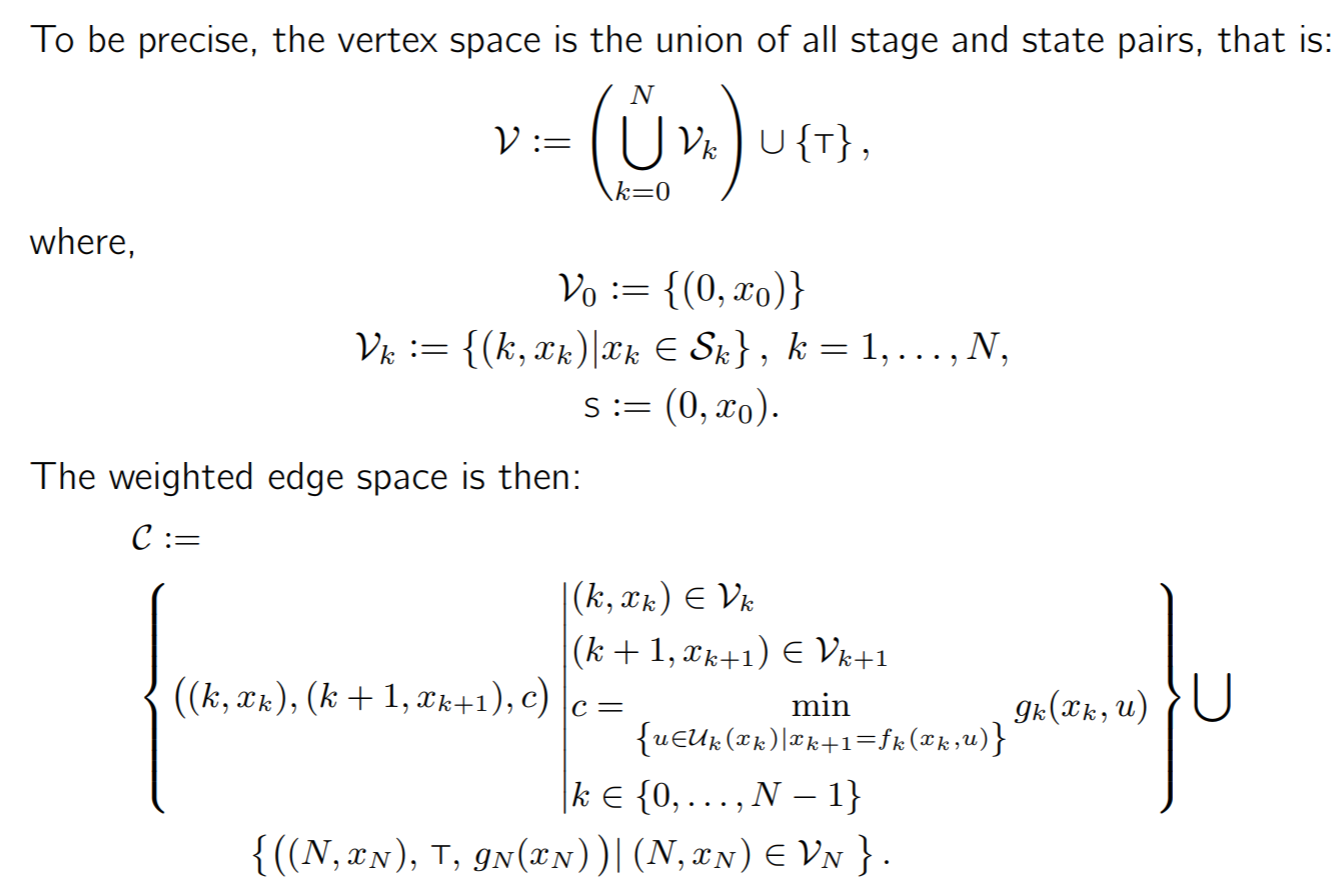
\includegraphics[width=\linewidth]{pictures/DFS_SP_description.png}
\end{Figure}

Stage:0,...,N; state:1,...n

\begin{Figure}
	\centering
	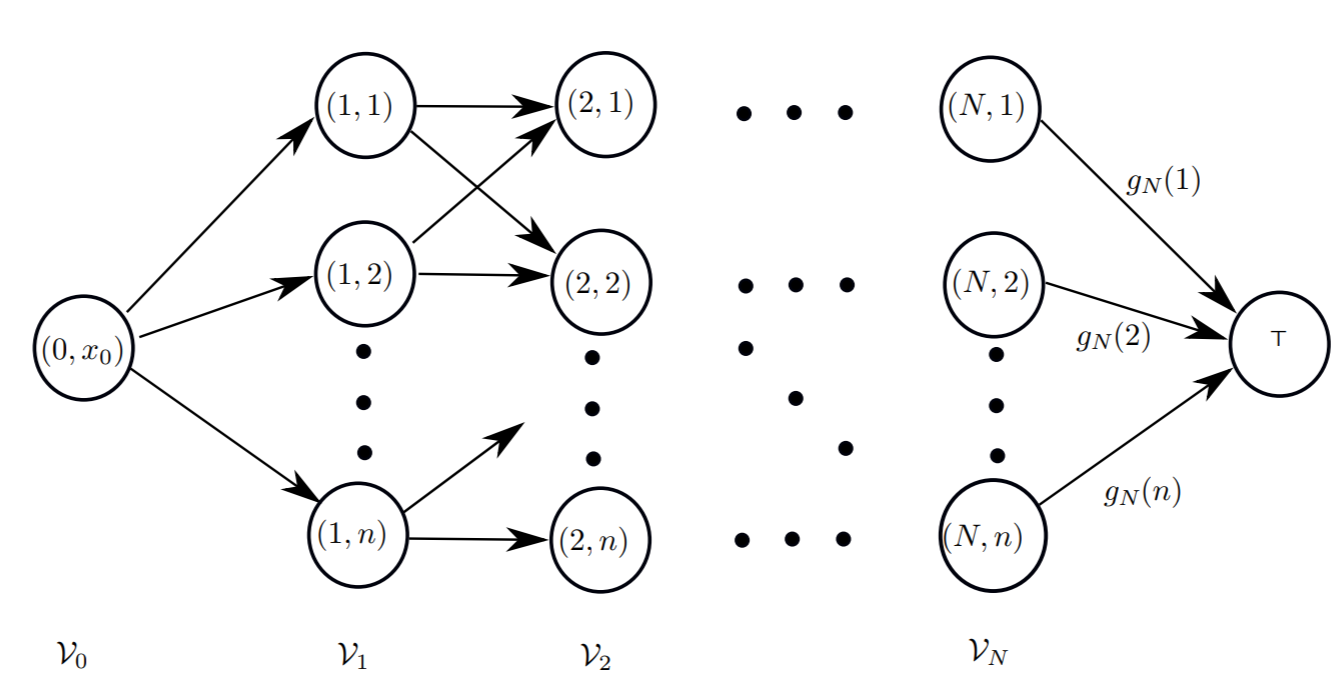
\includegraphics[width=\linewidth]{pictures/DFS_SP.png}
\end{Figure}

\textbf{SP $\rightarrow$ DFS}

\begin{Figure}
	\centering
	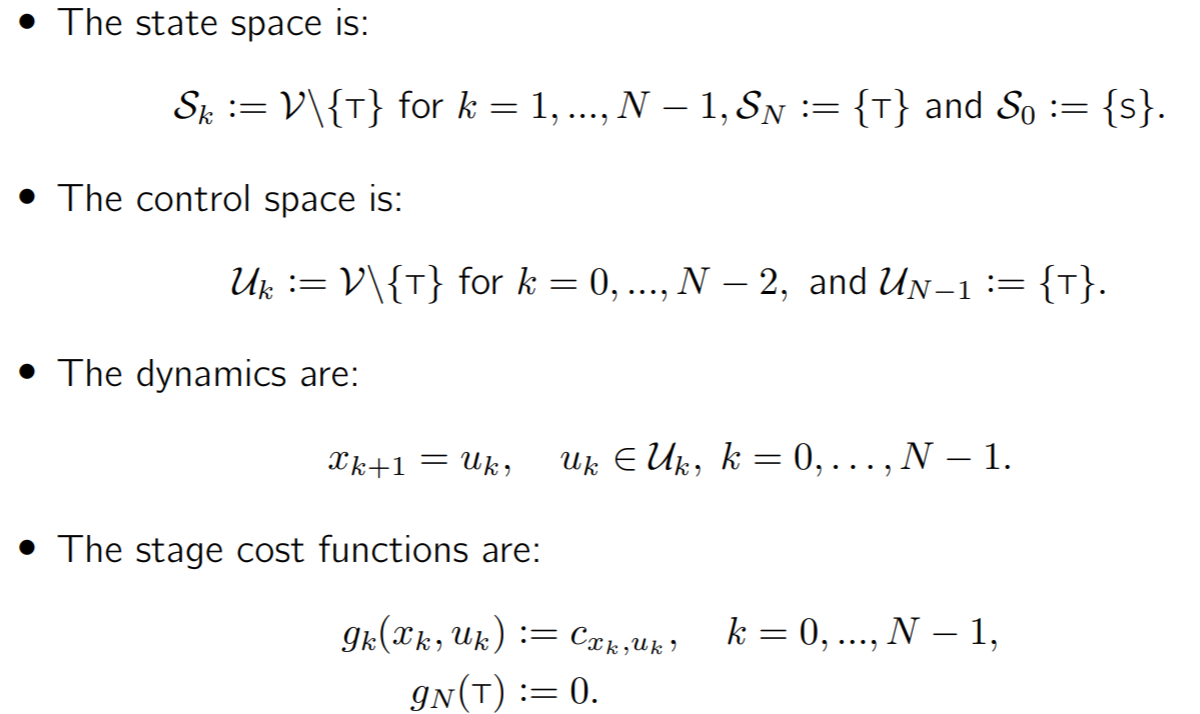
\includegraphics[width=\linewidth]{pictures/SP_DFS.png}
\end{Figure}
\begin{Figure}
	\centering
	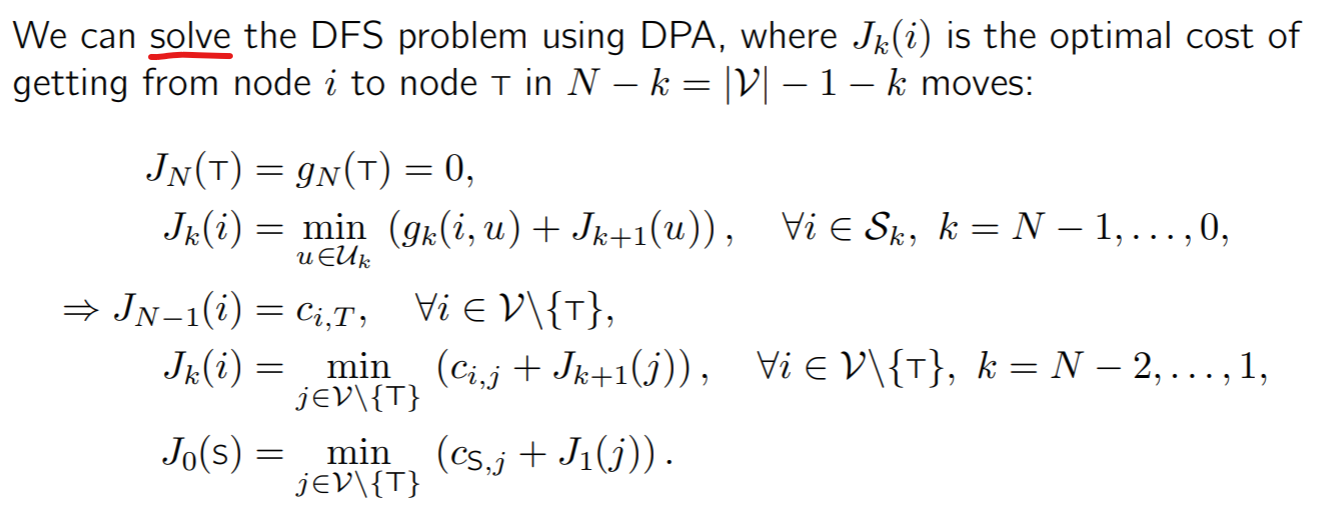
\includegraphics[width=\linewidth]{pictures/SP_DFS_2.png}
\end{Figure}

*Remark: We can terminate the algorithm early if $J_k(i) = J_{k+1}(i)$ for all $i\in V \backslash \{T\}$\\


\textbf{Hidden Markov Models: }
$\bullet$Dynamics: $x_{k+1} = w_k, x_k \in S, $
$P_{ij} = p_{w|x}(j|i), \forall i,j \in S$
the distributions $p_{x_0}$ and $p_{w|x}$ are given (\textit{Markov Chain})\\
$\bullet$ Measurement: $M_{ij}(z) = p_{z|x,w}(z|i,j)$ (given, \textit{likelihood function})\\
$\bullet$ Objective: Given a measurement sequence $Z_1 = (z_1,...,z_N)$, find the "most likely" state trajectory $X_0=(x_0,...,x_N) = \underset{X_0}{argmax} p(X_0|Z_1)$

\textbf{Viterbi Algorithm: }\\
$p(X_0, Z_1) = p(X_0|Z_1)p(Z_1) \rightarrow argmax p(X_0,Z_1)$ \\
$p(X_0,Z_1) = p(x_0) \prod_{k=1}^{N} P_{x_{k-1}x_k}  M_{x_{k-1}x_k}(z_k)$\\
$\Longrightarrow \underset{X_0}{minimize}(c_{S,(0,x_0)} + \sum_{k=1}^{N} c_{(k-1,x_{k-1}), (k,x_k)})$\\


%\[ c_{S,(0,x_0)} = \left\{ \begin{array}{ll}
%	-ln(p(x_0)) & \mbox{if $ p(x_0) > 0$};\\
%	\infty & \mbox{if $p(x_0) = 0$}.\end{array} \right. \] 
%
%\[ c_{(k-1,x_{k-1}),(k,x_k)} = \left\{ \begin{array}{ll}
%	-ln(P_{x_{k-1}x_k}M_{x_{k-1}x_k}(z_k)) & \mbox{if $ P_{x_{k-1}x_k}M_{x_{k-1}x_k}(z_k) > 0$};\\
%	\infty & \mbox{if $P_{x_{k-1}x_k}M_{x_{k-1}x_k}(z_k) = 0$}.\end{array} \right. \] 

\begin{Figure}
	\centering
	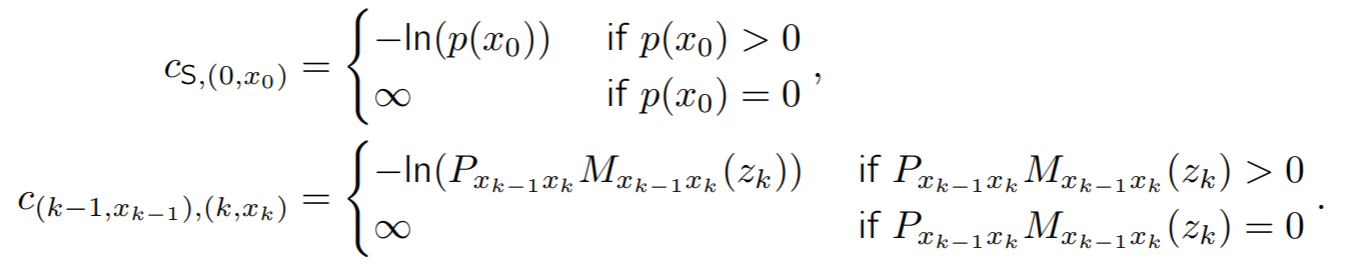
\includegraphics[width=\linewidth]{pictures/Viterbi_1.png}
\end{Figure}
\begin{Figure}
	\centering
	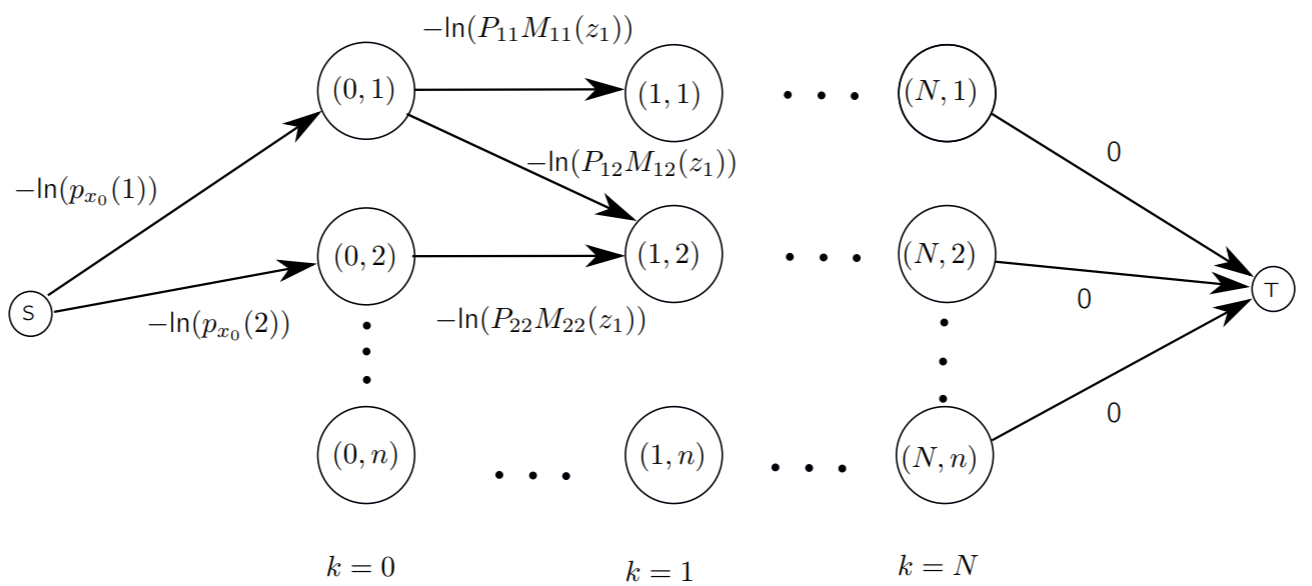
\includegraphics[width=\linewidth]{pictures/Viterbi_2.png}
\end{Figure}

% Lecture 8

\textbf{Label correcting methods:}\\
\begin{Figure}
	\centering
	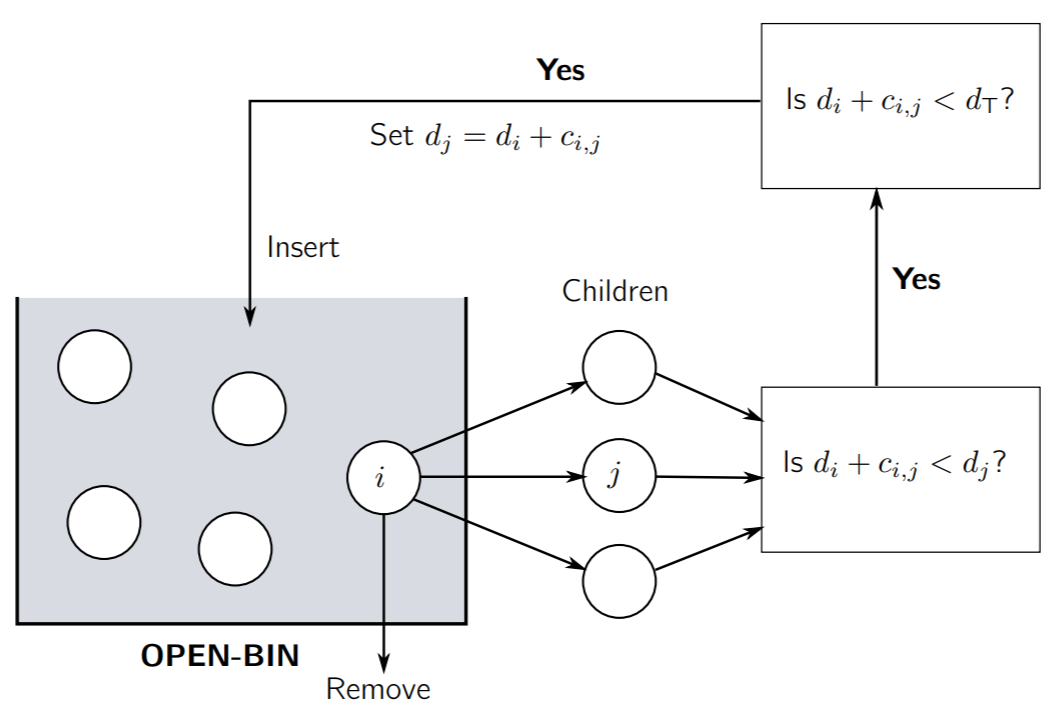
\includegraphics[width=\linewidth]{pictures/LCM.png}
\end{Figure}
Initialization: Place node S in OPEN, set $d_S=0, d_j=\infty \forall j\in V \backslash\{S\}$\\
*Theorem:  If there exists at least one finite cost path
from S to T, then the LCA terminates with $d_T = J_{Q^{*}}$. Otherwise, the LCA termimnates with $\infty$.

$\bullet$ \textbf{Depth-First Search} or “last in, first out” strategy, that is, a node is always removed from the top of the OPEN bin and each node entering OPEN is placed at the top. It is often implemented as a stack.\\
$\bullet$ \textbf{Breadth-First Search} or “first in, first out” strategy; that is, a node is always removed from the top of the OPEN bin and each node entering OPEN is placed at the bottom. It is often implemented as a queue.\\
$\bullet$ \textbf{Best-First Search (Dijkstra’s Algorithm)}: At each iteration, the node
that is removed from OPEN is the node $i^{*}$ where $d_{i^{*}} = \underset{i \in OPEN}{min} d_i$, i.e. remove the node that currently has the best label.\\
$\bullet$ \textbf{$A^{*}$-algorithm:}in step 2 of LCA, we strengthen requirement of a node j being admitted to OPEN from $d_i+c_{i,j} < d_T$ to $d_i+c_{i,j}+h_j < d_T$, where $h_j$ is some positive lower bound on the cost to get from node j to T (heuristic).

% Lecture 9
\textbf{Deterministic Continuous Time Model:}\\
$\bullet$ Dynamics: $\dot{x}(t) = f(x(t),u(t)), 0 \leq t \leq T$,\\
where $x(t) \in S=\mathbb{R}^n$ and $u(t)\in U \subset \mathbb{R}^m$\\
$\bullet$ Feedback control law: let $\mu(.,.)$ be an \textit{admissible control law} that maps state $x \in S$ at time $t$ to control input $u(t)$: $u(t) = \mu (t,x), u(t)\in U, \forall t \in [0,T], \forall x\in S$\\
$\bullet$ Cost: $J_{\mu}(0,x) = h(x(T)) + \int_{0}^{T}g(x(\tau),u(\tau)) d\tau$\\
$\bullet$ Objective: Construct an optimal feedback control law $\mu^{*} \in \Pi$ s.t. $J_{\mu^{*}} (0,x) \leq J_{\mu} (0,x), \forall \mu \in \Pi, \forall x \in S$\\

\textbf{Assumption for existence and uniqueness: }\\
For any admissible control law $\mu$, initial time $t \in [0,T]$  and initial condition $x(t) \in S$, there exists a unique state trajectory $x(\tau)$ that satisfied: $\dot{x}(\tau) = f(x(\tau),u(\tau)), t \leq \tau \leq T$

*required for the problem to be well-defined

\textbf{Hamilton-Jacobi-Bellman (HJB) Equation}\\
$ 0 = \underset{u \in U}{min} [g(x,u) + \frac{\partial J^{*}(t,x)}{\partial t} + \frac{\partial J^{*}(t,x)}{\partial x}f(x,u)]$, $\forall t \in [0,T], \forall x \in S$, subject to terminal state $J^{*}(T,x) = h(x)$\\

\begin{Figure}
	\centering
	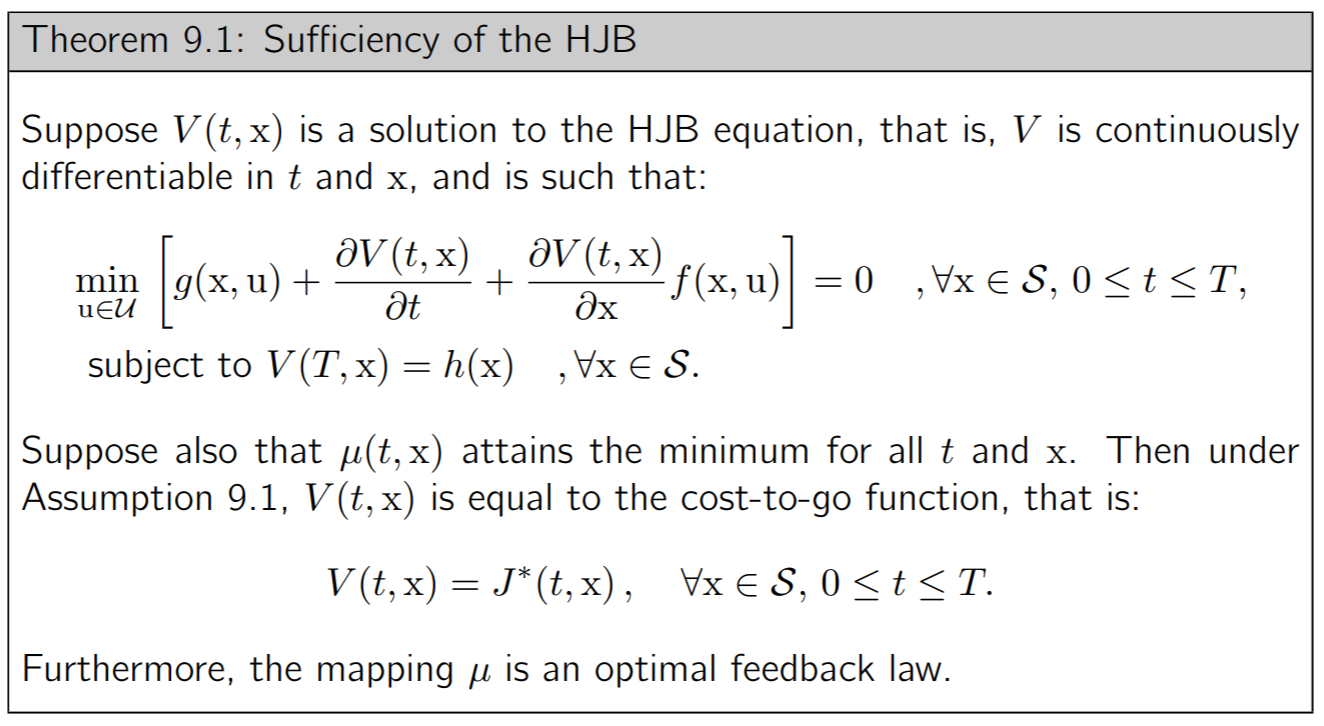
\includegraphics[width=\linewidth]{pictures/HJB.png}
\end{Figure}

*The optimal cost-to-go function may sometimes be not differentiable w.r.t. x or t at some places, thereby not satisfying the HJB. $\rightarrow$ HJB is in general not a necessary condition for optimality, but it is sufficient.
In this case we may use generalized solutions like piecewise continuous function to apply HJB.

% Lecture 10
\textbf{Partial Derivative} of $F(x,t)$ is $\frac{\partial J(t,x)}{\partial t}$\\
Partial Derivative of $F(x(t),t)$ is
$\frac{\partial J(t,x(t))}{\partial t} = \frac{\partial J(t,x)}{\partial t}|_{x=x(t)} + \frac{\partial J(t,x)}{\partial x}|_{x=x(t)} \frac{\partial x(t)}{\partial t}$\\
\textbf{Total derivative} of $F(x(t),t)$ is
$\frac{\partial J(t,x(t))}{\partial t} = \frac{\partial J(t,x)}{\partial t}|_{x=x(t)} + \frac{\partial J(t,x)}{\partial x}|_{x=x(t)} \frac{dx(t)}{dt}$

\textbf{Lemma:}\\
$\frac{\partial (\underset{u\in U}{min} F(t,x,u))}{\partial t} = \frac{\partial F(t,x,u)}{\partial t}|_{u=\mu^{*}(t,x)}$\\
$\frac{\partial (\underset{u\in U}{min} F(t,x,u))}{\partial x} = \frac{\partial F(t,x,u)}{\partial x}|_{u=\mu^{*}(t,x)}$\\

\begin{Figure}
	\centering
	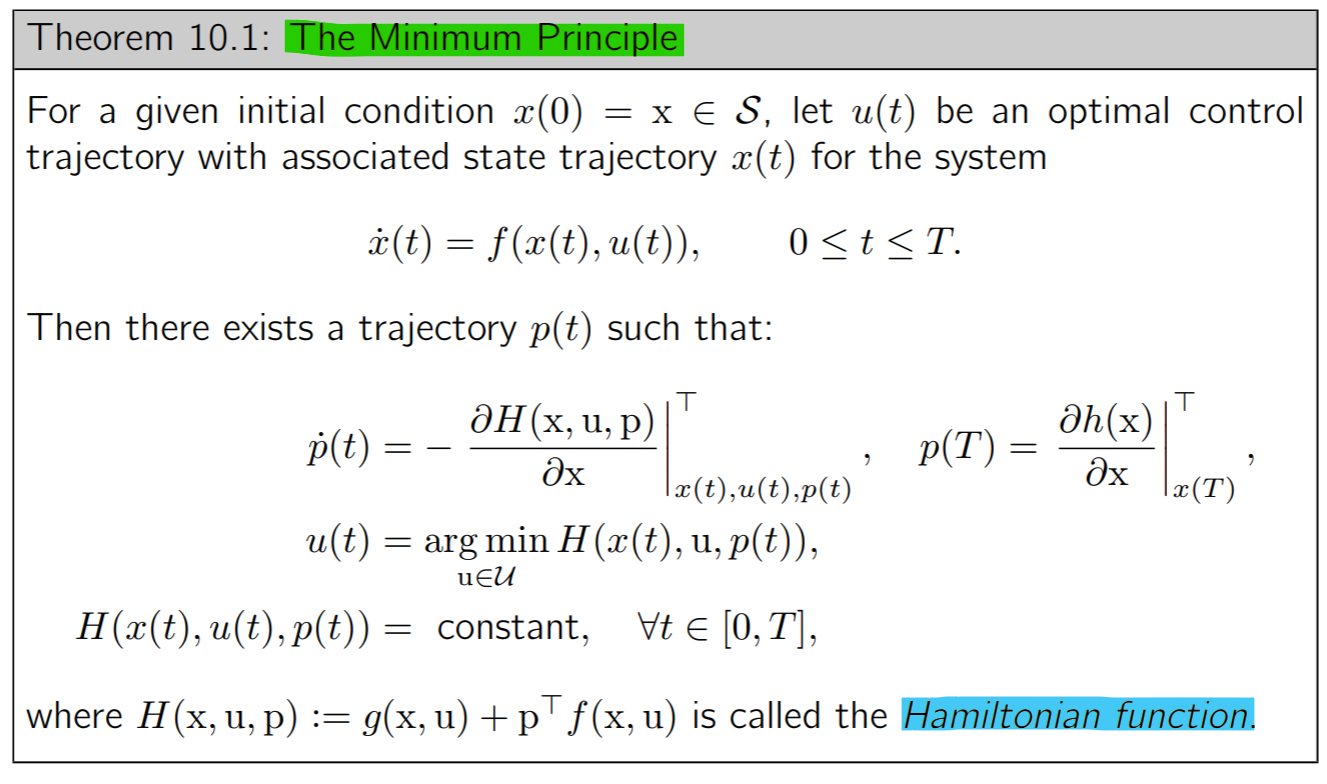
\includegraphics[width=\linewidth]{pictures/MP.png}
\end{Figure}
*1.$p(t) = \frac{\partial J(t,x)}{\partial x}^T $\\

2.The Minimum Principle provides necessary conditions for optimality. If a
control trajectory satisfies these conditions, it is not necessarily optimal.
\\

3.In general, if the Hamiltonian is linear in u, the maximum or minimum of the
Hamiltonian can only be attained on the boundaries of $U$. The resulting control trajectory is known as \textbf{bang-bang control}.\\

4. HJB is sufficient condition for optimality and the Minimum Principle is necessary condition.\\

\begin{Figure}
	\centering
	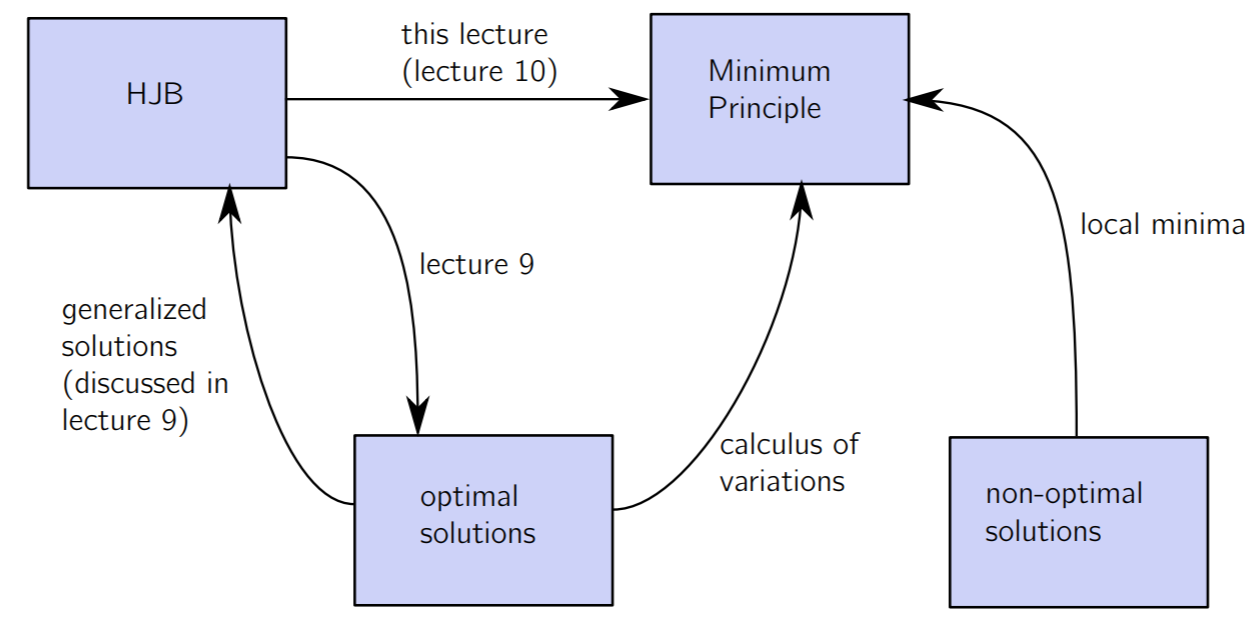
\includegraphics[width=\linewidth]{pictures/MP2.png}
\end{Figure}

% Lecture 11

\textbf{Fixed Terminal State:}\\
Instead of using $p(T)$, we use $x(T)$\\
$\dot{x}(t) = f(x(t),u(t)), x(0)=x_0, x(T)=x_T,$ \\
$ \dot{p}(t) = - \frac{\partial H(x,u,p)}{\partial x}|^T_{x(t),u(t),p(t)}$\\
*if only some of terminal states are fixed, then use them $x_i(T) = x_{T,i} , \forall i \in I$, for the other unfixed states, still use $p_j(T) = - \frac{\partial h(x)}{\partial x_j}|_{x(T)}, \forall j \notin I$\\

\textbf{Free Initial State:}\\
If $x_0$ is not given, instead, an additional cost $l(x(0))$ is given, total cost = $l(x(0)) + J(0,x(0))$, \\
then we use $p(0) = -\frac{\partial l(x)}{\partial x}|^T_{x(0)} $ instead of  $x_0$\\

\textbf{Free Terminal Time:}\\
Suppose the initial state and/or the terminal state are given, but the terminal time T is free.\\
In this case, $p(T) \rightarrow x_T$ and $H(x(t),u(t),p(t))=0$ instead of const.\\

\textbf{Time Varying System:}\\
$\dot{x}(t)=f(x(t),u(t),\textbf{t}),$ \\ 
cost $=h(x(T)) + \int_{0}^{T}g(x(\tau),u(\tau), \tau) d\tau$\\
Introduce $y(t) = t, y(0)= 0, \dot{y}(t)=1 $\\
$z(t) = (x(t),y(t))$\\

$ \dot{z}(t) = \begin{bmatrix}
	f(x(t),u(t),y(t))\\ 
	1
\end{bmatrix} = \bar{f}(z(t),u(t))$,\\
%cost $=\bar{h}(x(T)) + \int_{0}^{T}\bar{g}(x(\tau),u(\tau), \tau) d\tau$\\  
hence, the Hamiltonian: $\bar{H}(z,u,\bar{p}) = \bar{g}(z,u) + \bar{p}^T\bar{f}(z,u) $ \\ 
$= g(x,u,y) + p^T f(x,u,y) + q = H(x,u,p,y) + q$\\
with $z = (x,y)$ and $\bar{p}(t) = (p(t),q(t))$\\
Hence, conditions of the Minimum Principle:\\
$\dot{p}(t) = - \frac{\partial H(x,u,p)}{\partial x}|^T_{x(t),u(t),p(t)}$\\
$p(T) = \frac{\partial h(x)}{\partial x}|^T_{x(T)}$\\
$u(t) = \underset{u\in U}{argmin} H(x(t),u,p(t))$\\
*$\dot{q}(t) = - \frac{\partial \bar{H}(x,u,p)}{\partial t}|^T_{z(t),u(t),\bar{p}(t)}$\\
*$\bar{H}(z(t),u(t),\bar{p}(t)) = H(x,u,p,t) + q(t) = $ constant\\

Note that the only difference between the TI and the TV cases is that the Hamiltonian in the latter one need not be constant along the optimal trajectory.
\\

\textbf{Singular Problems}\\
In some cases, the Minimum Principle condition $u(t) = \underset{u\in U}{argmin} H(x(t),u,p(t),t)$ is insufficient to determine $u(t)$ for all $t$, because the values of $x(t)$ and $p(t)$ are such that $H(x(t),u,p(t))$ is independent of $u$ over a nontrivial interval of time.\\
*Their optimal trajectories consist of portions, called \textbf{regular arcs}, where $u(t)$ can be determined from the minimum principle condition, and other portions, called \textbf{singular arcs}, which can be determined from the condition that the Hamiltonian is independent of u.





\end{multicols*}


\end{document}